\documentclass[border=4pt]{standalone}
\usepackage[T5,T1]{fontenc}
\usepackage{mathptmx}
\usepackage{tikz}
\usetikzlibrary{positioning,arrows.meta,fit,backgrounds,calc}
\definecolor{ink}{HTML}{13294B}
\definecolor{teal}{HTML}{1C7293}
\definecolor{amber}{HTML}{E8A33D}
\tikzset{
  >={Stealth[length=2mm]},
  comp/.style={draw=ink!70, rounded corners=2pt, fill=white, align=center, text width=#1,
               inner sep=3pt, minimum height=9.5mm, font=\footnotesize},
  comp/.default=3.3cm,
  frame/.style={draw=teal, rounded corners=4pt, fill=teal!6, inner sep=7pt},
  oframe/.style={draw=amber!90!black, rounded corners=4pt, fill=amber!10, inner sep=7pt},
  stepbadge/.style={circle, fill=ink, text=white, inner sep=0.8pt, minimum size=4.2mm, font=\scriptsize\bfseries},
  flow/.style={->, draw=ink, thick},
  lab/.style={font=\scriptsize, align=center, fill=white, inner sep=1.2pt},
  art/.style={->, draw=ink!55, dashed},
}

\newcommand{\vi}[1]{{\fontencoding{T5}\selectfont #1}}
\newcommand{\Ldet}{Yes/no detector\\ \scriptsize rule-based, \texttt{core.py}}
\newcommand{\Lprompt}{Prompt builder\\ \scriptsize \texttt{builder.py}, shared with training and evaluation}
\newcommand{\Lmodel}{Qwen2.5-VL-3B-Instruct\\ \scriptsize 4-bit NF4 + LoRA adapter SH (PEFT); greedy, or first-token margin vs.\ $\tau^*$}
\newcommand{\Lconf}{Confidence level\\ \scriptsize High / Medium / Low}
\newcommand{\Lprep}{Image preparation\\ \scriptsize original file, EXIF rotation,\\ \scriptsize $\le$\,6,000\,px}
\newcommand{\Lcache}{OCR prefetch and cache\\ \scriptsize SHA-1 key, up to 32 images}
\newcommand{\Lshow}{Presentation\\ \scriptsize answer, level,\\ \scriptsize numbered OCR boxes}
\newcommand{\Lpdet}{PaddleOCR\\ \scriptsize text detection}
\newcommand{\Lvrec}{VietOCR\\ \scriptsize text recognition}
\newcommand{\Lmainp}{Main process (Python, PyTorch)}
\newcommand{\Lbackend}{Backend \texttt{core.py}}
\newcommand{\Lui}{Web interface \texttt{app.py} (Gradio)}
\newcommand{\Locrp}{OCR process\\ \texttt{ocr\_worker.py}}
\newcommand{\Luser}{User (web browser)}
\newcommand{\Lart}{\textbf{Read-only artefacts}\\[2pt] SH adapter\\ (SHA-256 checked)\\[1pt] \texttt{qwen\_lora.yaml}\\[1pt] verified thresholds (W13 summary)}
\newcommand{\Limage}{image}
\newcommand{\Lquestion}{question}
\newcommand{\Ljson}{JSON lines (stdin/stdout)}
\newcommand{\Locrlines}{OCR lines}
\newcommand{\Lanswer}{answer, level, OCR evidence}
\begin{document}
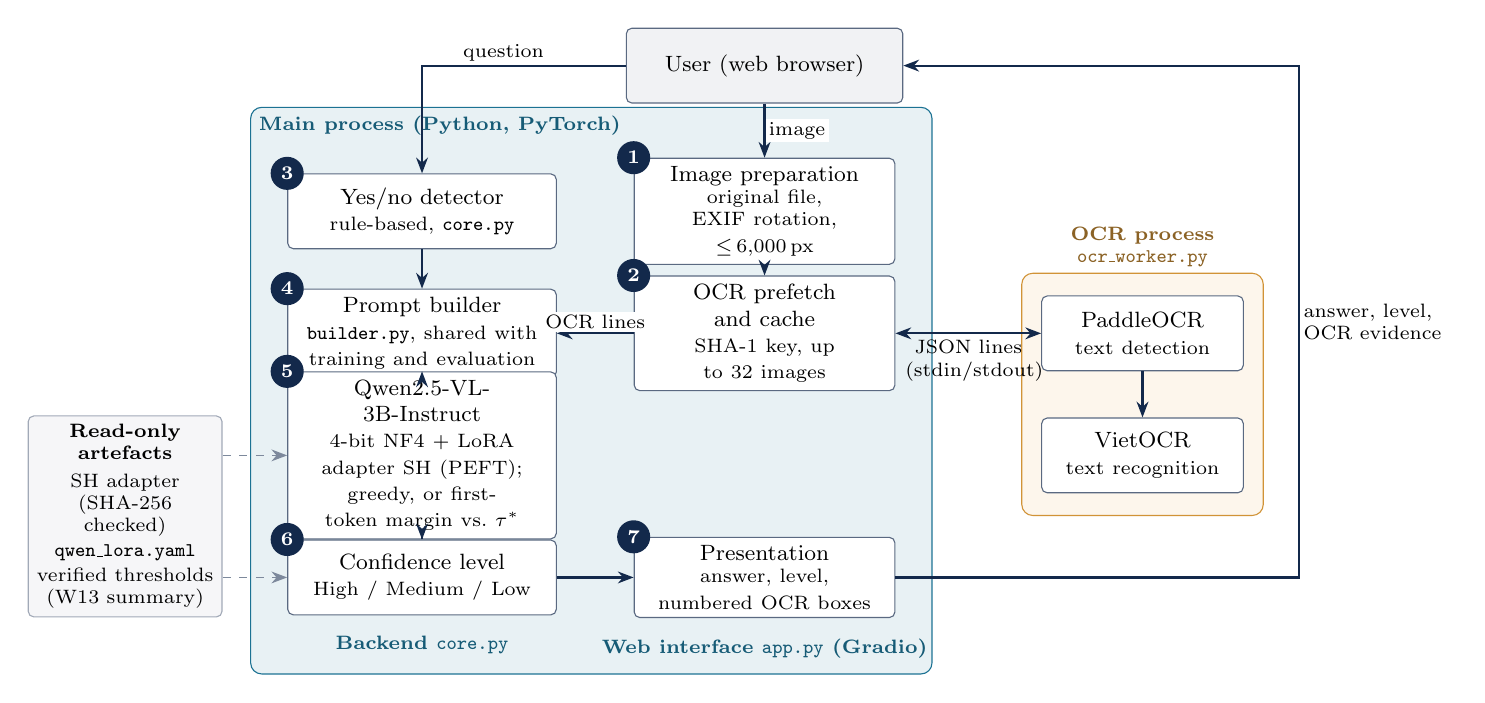
\begin{tikzpicture}
% rows: y0 = 0, y1 = -1.55, y2 = -3.1, y3 = -4.65
% ---- backend column (core.py)
\node[comp=3.2cm] (det)    at (3.4, 0)     {\Ldet};
\node[comp=3.2cm] (prompt) at (3.4,-1.55)  {\Lprompt};
\node[comp=3.2cm] (model)  at (3.4,-3.1)   {\Lmodel};
\node[comp=3.2cm] (conf)   at (3.4,-4.65)  {\Lconf};
% ---- interface column (app.py)
\node[comp=3.1cm] (prep)   at (7.75, 0)    {\Lprep};
\node[comp=3.1cm] (cache)  at (7.75,-1.55) {\Lcache};
\node[comp=3.1cm] (show)   at (7.75,-4.65) {\Lshow};
% ---- OCR process
\node[comp=2.35cm] (pdet)  at (12.55,-1.55) {\Lpdet};
\node[comp=2.35cm] (vrec)  at (12.55,-3.1)  {\Lvrec};
% ---- column frames
\begin{scope}[on background layer]
  \node[frame, fill=teal!4, draw=teal!60, inner sep=5pt, fit=(det)(conf)] (bf) {};
  \node[frame, fill=teal!4, draw=teal!60, inner sep=5pt, fit=(prep)(show)] (uf) {};
  \node[frame, fill=teal!10, draw=teal, inner xsep=8pt, inner ysep=14pt, yshift=-1pt, fit=(bf)(uf)] (mainf) {};
  \node[oframe, inner xsep=7pt, inner ysep=8pt, fit=(pdet)(vrec)] (ocrf) {};
\end{scope}
\node[font=\scriptsize\bfseries, text=teal!80!black, anchor=north west, inner sep=3pt] at (mainf.north west) {\Lmainp};
\node[font=\scriptsize\bfseries, text=teal!80!black, anchor=north, inner sep=2pt] at (bf.south) {\Lbackend};
\node[font=\scriptsize\bfseries, text=teal!80!black, anchor=north, inner sep=2pt] at (uf.south) {\Lui};
\node[font=\scriptsize\bfseries, text=amber!60!black, anchor=south, align=center, inner sep=2pt] at (ocrf.north) {\Locrp};
% ---- user
\node[comp=3.3cm, fill=ink!6] (user) at (7.75, 1.85) {\Luser};
% ---- artefacts
\node[comp=2.25cm, fill=ink!4, draw=ink!40, text width=2.25cm, anchor=east, font=\scriptsize] (art) at ($(mainf.west |- model)!0.5!(mainf.west |- conf)+(-0.35,0)$) {\Lart};
% ---- step badges
\foreach \n/\s in {prep/1, cache/2, det/3, prompt/4, model/5, conf/6, show/7}
  \node[stepbadge] at (\n.north west) {\s};
% ---- flows
\draw[flow] (user) -- node[lab, right] {\Limage} (prep);
\draw[flow] (user.west) -| node[lab, pos=0.3, above] {\Lquestion} (det.north);
\draw[flow] (prep) -- (cache);
\draw[flow, <->] (cache.east) -- node[lab, below=1pt, text width=1.6cm, fill=none] {\Ljson} (pdet.west);
\draw[flow] (pdet) -- (vrec);
\draw[flow] (cache.west) -- node[lab, above] {\Locrlines} (prompt.east);
\draw[flow] (det) -- (prompt);
\draw[flow] (prompt) -- (model);
\draw[flow] (model) -- (conf);
\draw[flow] (conf.east) -- (show.west);
\draw[flow] (show.east) -- ($(show.east -| ocrf.east)+(0.45,0)$) |- node[lab, pos=0.25, right, text width=1.9cm, align=left] {\Lanswer} (user.east);
% ---- artefacts (dashed)
\draw[art] (art.east |- model) -- (model.west);
\draw[art] (art.east |- conf)  -- (conf.west);
\end{tikzpicture}

\end{document}
